\documentclass[11pt]{article}





\usepackage[margin=1.25in]{geometry}
\usepackage{graphicx}
\graphicspath{ {.} }
\usepackage{imakeidx}

\makeindex[columns=3, title=Alphabetical Index, intoc]


\begin{document}

\begin{titlepage}

\title{%
  Secure Game \\
  \large  Security of Information and Organizations Project 2\\}

\author{Rafael Remígio 102435 \\ Bruno Moura 97151\\ João Correia 104360}

\maketitle

\vfill
\begin{center}

	Departamento de Electrónica, Telecomunicações e Informática\\
       Universidade de Aveiro\\ Year 2022/2023
\end{center}



\end{titlepage}

\tableofcontents

\clearpage

\section{Introduction}
The proposed assignment entails the designing and implementation of a robust protocol for handling a simplified game of bingo played on a distributed system. 
\\ Instead of trusting an authoritative party to authenticate messages and certify that the game is to be played fairly, it is assumed that every playing entity may cheat and as such trust is instead placed on the security mechanisms in place. To this end, we used \emph{asymmetric and symmetric cryptography}, \emph{digital signatures}, emph{smart cards} and \emph{certificates}.
\\This document aims to document the implementation and architecture of the distributed system and protocol, as well as the design decisions behind their creation.

\pagebreak

\section{Entities}
The system comprises of three types of entities, the Playing Area, Caller and a Player.
\\ \\ {\Large \textbf{Playing Area}} \par
The first is the playing area, a secure playing field. It does not interfere with the game directly, but instead handles authentication and authorization. \\
Players and callers all interact with the playing area instead of with each other directly. Its job is to verify messages and forward them around.
It possesses a RSA 128 bit asymmetric key pair for signing messages.
\\ \\ {\Large \textbf{Player}} \par
The second type of entity is the player. As the name implies, these are the entities that will actually play the game and are eligible for winning and losing. There must be at least two players per game. \\
During the game, the players will generate a card of numbers from the deck provided by the caller. The player whose card gets filled first wins, as per bingo rules. \\ It possesses a Portuguese citizen card capable of signing documents, a RSA 128 bit asymmetric key pair and a AES 128 bit symmetric key. Their use will be explained later own.
\\ \\ {\Large \textbf{Caller}} \par
Lastly, the third and final type of entity is the caller, of which there is only one per game. The caller is responsible for generating the deck, an ordered list of numbers that will simulate the draw of balls of a traditional bingo game.
\\The caller possesses the same keys as the player. In fact, a caller is functionally identical to an user during the authentication and registration process. So whenever the term user is used, what is being said applies both to players and callers.


\section{Walk-through}
This section will outline the steps the system takes for running a game of bingo. Further details on the protocol messages will be covered in the next section. 

\subsection{Authentication}
The game cannot start until there are enough users and a caller connected, authenticated and registered to the playing area. After connecting to the playing area via a web socket, the next step for a user is to authenticate themselves. \\
The authentication entails verifying that the user in question is a Portuguese citizen, as proved by their possession of a Portuguese citizen card (CC) and it’s PIN. \\ The authentication process is done through a Challenge-Response approach, in which a four step handshake is done to successfully authenticate a user.
\\ The handshake goes as follows:

\begin{enumerate}
  \item The user asks the \emph{Playing Area} to be authenticated by sending a authentication message containing their CC’s public key.
  \item The \emph{Playing Area} sends a nonce to the user as a challenge.
  \item The \emph{user} encrypts the challenge with their CC’s private key and sends it back to the playing area.
  \item The user verifies that the response it got matches the nonce and public key. If so, a message is sent to the \emph{user} letting them know they are authenticated.
\end{enumerate}
The nonce consists of a string of random characters of variable length (by default, 14). It is wise to not set this length too low otherwise repeated challenges might occur and adversaries may then employ replay attacks to bypass authentication. \\ Authenticated users are not ready to join the game as of yet. For that, they must be registered. At this step, the playing area merely recognizes them as a Portuguese system citizen. They can now, however, ask the playing area for message logs and a list of registered users. \\ Also, the playing area possesses a set of CC public keys that are reserved for callers. As such, what determines if a user will be a player or a caller.

\subsection{Registration}
The next and final step for a user to be fully ready to participate in the game is the registration process. It’s purpose is to establish what is the public key that will be used during the game, as the CC’s key pair is only used for authentication purposes. The user must also register himself a nickname to aid identification by humans. \\ The registration also is done through a handshake.
\begin{enumerate}
	\item The user asks the playing area to be registered by sending a registration message. The message contains the public key from the key pair just now generated (the playing key), their nickname, the CC public key and a signature.
	\item The playing area receives the message and validates the signature. If it’s valid, the user is now registered. The playing area sends the message back confirming the registration.
\end{enumerate}
After the registration, the playing area follows up with a message informing about some data about the game – namely the user’s sequence (sequential ID), the size of the cards and the size of the deck.
\\At this point, the playing area will automatically start the game once a caller and a variable amount of players (default 2) have registered themselves. Once a user is registered, every other registered user is notified by the playing area (the same also happens if a registered user disconnects)
During earlier stages of development, we considered merging the authentication and registration; The user would provide their nickname, the public key that will be used for the game, their CC’s public key and a CC digital signature.\\
We ended up opting for a Challenge-Response authentication approach to prevent a particular kind of attack, in which an adversary somehow gets a hold of the private key of a key pair used by a victim in a game they were in. They can then reuse the authentication message used in the original game to play as the victim as long as they use the compromised key pair as playing key
\begin{center}
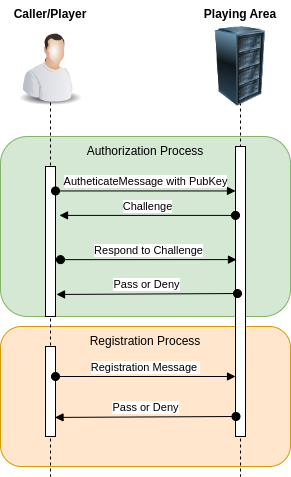
\includegraphics{AuthenticateUML.png}
\end{center}
\clearpage

\subsection{Deck and Card Generation}


\end{document}
